% Created 2020-11-14 Sat 16:22
% Intended LaTeX compiler: pdflatex
\documentclass[a4paper]{article}
\usepackage[utf8]{inputenc}
\usepackage[T1]{fontenc}
\usepackage{graphicx}
\usepackage{grffile}
\usepackage{longtable}
\usepackage{wrapfig}
\usepackage{rotating}
\usepackage[normalem]{ulem}
\usepackage{amsmath}
\usepackage{textcomp}
\usepackage{amssymb}
\usepackage{capt-of}
\usepackage[greek, ngerman, germanb]{babel}
\usepackage{hyperref}
\usepackage{minted}
\renewcommand\refname{Quellen}
\usepackage{textgreek}
\usemintedstyle{emacs}
\newcommand{\printbibliography}[1][h]{\bibliographystyle{alpha}\bibliography{referenzen}}
\usepackage[left=2.5cm,right=2cm,top=1.5cm,bottom=1cm,includeheadfoot]{geometry}
\author{Johannes Brauer}
\date{2020-11-14 Sat 16:22}
\title{Nutzung von React-Frameworks\\\medskip
\large Dozenteneinsatzplanung mit re-frame}
\hypersetup{
 pdfauthor={Johannes Brauer},
 pdftitle={Nutzung von React-Frameworks},
 pdfkeywords={},
 pdfsubject={},
 pdfcreator={Emacs 25.3.50.1 (Org mode 9.3.7)}, 
 pdflang={Germanb}}
\begin{document}

\maketitle

\section*{Einstieg}
\label{sec:org469c1ce}
\begin{itemize}
\item Funktional-reaktive Programmierung keine neue Idee
\cite{Wan2000Functional}.
\begin{itemize}
\item Nutzung einer internen (Haskell) DSL
\end{itemize}
\item Populär geworden durch das Javascript-Framework \emph{\href{https://reactjs.org}{React}} von Facebook
\item Bevorzugte Verwendung für die Erstellung von Einzelseiten-Webanwendungen (single
page applications)
\item Nutzung durch die Clojurescript-Adaption \emph{\href{https://github.com/reagent-project/reagent}{Reagent}} für
\href{https://johbra.github.io/dep/}{Dozenteneinsatzplanung} (mit \href{https://drive.google.com/open?id=1ZR3xy5EXyZfarY7tpM-t8LH1V5gfLO3F}{Erfahrungsbericht})
\end{itemize}
\section*{Merkmale von FRP}
\label{sec:org2f355a1}
\subsection*{Reaktive Systeme}
\label{sec:orgcd2f3b6}
\begin{itemize}
\item ereignis-getriebene Anwendungen
\item kontinuierliche Interaktion mit ihrer Umgebung
um z.~B.
\begin{itemize}
\item die Aktualisierung des Anwendungszustands,
\item die Anzeige von Daten zu erledigen
\item interaktivste Komponente einer Anwendung häufig die
Benutzungsoberfläche: Reaktion auf verschiedene Ereignisse wie
Mausklicks, Tastatureingaben oder die Betätigung von Schaltflächen
\end{itemize}
\item Herausforderungen reaktiver Systeme:
\begin{itemize}
\item inhärent nebenläufig:
\begin{itemize}
\item Reaktion auf asynchron auftretende Ereignisse verschiedener Herkunft
\item Darstellung sich verändernder Daten
\end{itemize}
\end{itemize}
\end{itemize}
\begin{itemize}
\item invertierte Kontrollstruktur:
\begin{itemize}
\item Anwendung steuert sich nicht selbst, sondern die Ermittlung der
nächsten auszuführenden Berechnung wird durch externe Ereignisse
oder Systeme bestimmt.
\item häufig anzutreffende Lösung: Bereitstellung von Routinen, sog.
Rückruffunktionen  (callback functions), die beim Auftreten
bestimmter Ereignisse aktiviert werden und in der Regel
zustandsändernde Operationen ausführen.
\item „Callback-Hölle“: viele isolierte Programmfragmente verändern
dieselben Daten
\end{itemize}
\item Die geschilderten Probleme legen nahe, funktionale
Programmiertechniken in Betracht zu ziehen.
\end{itemize}
\subsection*{Manifesto}
\label{sec:org3425ea1}
\href{https://www.reactivemanifesto.org}{The Reactive Manifesto} definiert Eigenschaften reaktiver Systeme.

Reaktive Systeme sind
\begin{description}
\item[{responsive}] reagieren „zeitnah”
\item[{resilient}] bleiben responsive auch im Fehlerfall
\item[{elastic}] bleiben responsive auch unter Last
\item[{message driven}] basieren auch asynchronem Nachrichtenaustausch
\end{description}
\subsection*{Schematische Darstellung interaktiver Anwendungen}
\label{sec:org78ee706}
Formulierung in einer internen DSL
\begin{minted}[]{scheme}
(big-bang state             ;; der Weltzustand
  {:on-tick  tick-handler   ;; tick-handler liefert bei jedem Zeittakt neuen state
   :on-key   key-handler    ;; key-handler berechnet aus state und key neuen state
   :on-mouse mouse-handler  ;; mouse-handler berechnet aus state, den Mauskoordinaten
                            ;; und der Mausaktion neuen stat
   :to-draw   render        ;; render verwandelt state in ein Bild (view)
   :stop-when end?}         ;; end? ermittelt aus state das Ende der Ausführung
   ...)
\end{minted}
\begin{itemize}
\item Die Handler, \texttt{render} und \texttt{end?} sind reine Funktionen.
\item Die Mutation von \texttt{state} ist in \texttt{big-bang} versteckt.
\item \href{file:///Users/jb/Google-Drive/Planung/Clojure-Script/big-bang/src/bb/my\_scetch.cljs}{Beispiel}
\end{itemize}
\subsection*{Bestandteile}
\label{sec:org67b543a}
\begin{itemize}
\item Events  (\texttt{:on-tick}, \texttt{:on-mouse}, \(\ldots\))
\item Handler (\texttt{tick-handler}, \texttt{mouse-handler},  \(\ldots\))
\item Views   (\texttt{render})
\end{itemize}
\subsection*{Eigenschaften von re-frame}
\label{sec:org5352780}
\begin{itemize}
\item Clojurescript-Framework auf Basis von Reagent/React für die
Programmierung und Benutzungsoberflächen von Single-Page-Applications
\item funktional
\item nutzt die Homoikonizitäts-Eigenschaft von Lisp:
\begin{quote}
You are programming in data. The functions which later transform
data, themselves start as data.
\end{quote}
\item \hyperref[sec:org3e38e09]{unidirektionaler Datenfluss}
\end{itemize}
\subsubsection*{Sechs Dominosteine}
\label{sec:org702b141}
\begin{description}
\item[{Event dispatch}] Event = Reaktion auf externe Ereignisse (Mausklick,
Websocket-Nachricht etc.)
\item[{Event handling}] Reaktion auf ein Event, notwendige Seiteneffekte werden ermittelt
\item[{Effect handling}] Seiteneffekte werden ausgeführt
\end{description}
Nach diesen drei Schritten ist der App-Zustand aktualisiert.
Die drei folgenden Dominosteine berechnen die Funktion \(v = f(z)\). Ein
View \(v\) ist eine Funktion \(f\) des App-Zustands \(z\).
\begin{description}
\item[{Query}] Extraktion und Aufbereitung der Daten aus \(z\)
\item[{View}] Rendern der Daten aus Query; Verwendung des \href{https://github.com/weavejester/hiccup}{hiccup}-Formats (HTML-DSL)
\item[{DOM}] Die DOM-Knoten des Web-Browsers werden durch Reagent/React
aktualisiert.
\end{description}
\paragraph*{Zusammenfassung}
\label{sec:orgca6811d}
\begin{center}
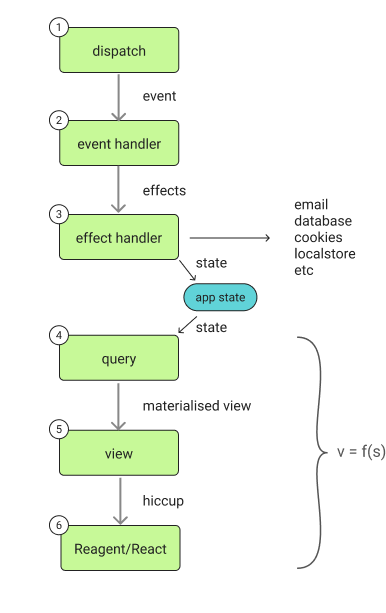
\includegraphics[width=.9\linewidth]{./Abbildungen/6dominoes.png}
\end{center}
\subsubsection*{App-Zustand}
\label{sec:org46bb7e4}
\begin{itemize}
\item ein globaler Zustand (single source of truth)
\item wird von re-frame automatisch angelegt: \\
\mintinline{clojure}{(def app-db  (reagent/atom {}))}
\item dient quasi als Hauptspeicherdatenbank
\item Alternativen
\begin{itemize}
\item \href{https://github.com/tonsky/datascript}{datascript}
\item \href{https://github.com/denistakeda/re-posh}{re-posh}
\end{itemize}
\end{itemize}
\subsubsection*{Code-Beispiele}
\label{sec:org302e5b4}
\paragraph*{Html-DSL}
\label{sec:orgb4b78a9}
\begin{itemize}
\item In View-Komponenten wird gemäß re-frame-Dokumentation das mit
Reagent bereitgestellte \href{https://github.com/weavejester/hiccup}{hiccup}-Format als HTML-DSL verwendet.
\item In der Dozenteneinsatzplanung wird überwiegend eine auf hiccup
aufbauende DSL benutzt: \href{https://github.com/day8/re-com}{re-com}. Re-com stellt
\begin{itemize}
\item die üblichen Widgets
\item Layout-Komponenten für die Anordnung von Widgets und
Layout-Komponenten (horizontale und vertikale Boxen) zur
Verfügung.
\end{itemize}
\item Beispiel für eine Schaltfläche:
\begin{nebeneinander}
\begin{minted}[]{clojure}
[button
    :class "btn-primary"
    :on-click #(plane-quartal)
    :label "Plane Quartal"]
\end{minted}
\end{nebeneinander}
\begin{nebeneinander}
\begin{center}

\includegraphics[width=.9\linewidth]{./Abbildungen/planebutton.png}
\end{center}
\begin{minted}[]{html}
<div class="rc-box display-flex rc-button-wrapper display-inline-flex" 
     style="flex-flow: inherit; flex: 0 0 auto; align-items: flex-start;">
  <button class="rc-button btn btn-primary" style="flex: 0 0 auto;">
    Plane Quartal</button>
</div>
\end{minted}
\end{nebeneinander}
\end{itemize}
\begin{clear}
\end{clear}
\begin{itemize}
\item Layout-Beispiel
\begin{small}
\begin{minted}[]{clojure}
[v-box
  :children [[box :child "Header"]
             [h-box
              :height "100px"
              :children [[box :size "70px" :child "Nav"]
                         [box :size "1" :child "Content"]]]
             [box :child "Footer"]]]
\end{minted}
\end{small}
resultiert in:
\begin{center}
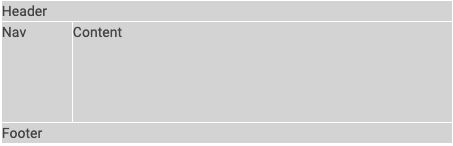
\includegraphics[width=.9\linewidth]{./Abbildungen/layout.png}
\end{center}
\end{itemize}

\paragraph*{View-Komponente für \href{http://localhost:9500/}{Auswahl von Geschäftsjahr und Quartal}}
\label{sec:org8ea9dc5}
\begin{minted}[linenos,firstnumber=1]{clojure}
(defn geschaeftjahr-quartal-form 
  "Die Auswahlboxen für Geschäftsjahr und Quartal und die Planungsschaltfläche."
  []
  (let [jahre @(rf/subscribe [:jahre])
        quartale @(rf/subscribe [:quartale])
        quartal @(rf/subscribe [:quartal])
        geschaeftsjahr @(rf/subscribe [:geschaeftsjahr])]
    [h-box :class "bg-light border-right" :gap "10px"
     :children
     [(select-box "Geschäftsjahr:" jahre geschaeftsjahr
                  #(rf/dispatch [:geschaeftsjahr (:key %)]))
      (select-box "Quartal:" quartale (quartal->string quartal)
                  #(rf/dispatch [:quartal (:key %)]))
      [button
       :class "btn-primary"
       :on-click #(plane-quartal)
       :label "Plane Quartal"]
      [button
       :class "btn-primary"
       :on-click #(neues-geschaeftjahr)
       :label "neues G-Jahr anlegen"] ]]))
\end{minted}
\begin{itemize}
\item In den Zeilen  gehts los
\end{itemize}
\section*{FRP vs. MVC}
\label{sec:org3a4ef0e}
\cite{Ferreira19}
\subsection*{Model-View-Controller}
\label{sec:org0e69eda}
\begin{itemize}
\item Datenfluss
\begin{center}
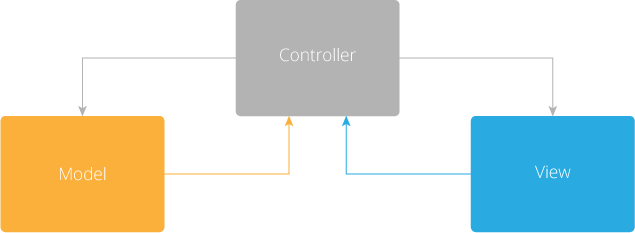
\includegraphics[width=.9\linewidth]{./Abbildungen/mvc.png}
\end{center}
\item repräsentiert das Single Responsibility Principle
\item komplexere Anwendungen (mit intensiver Benutzerinterkation)
überfordern den Controller:
\begin{itemize}
\item Verwaltung des Anwendungszustands
\item Mittler zwischen View und Model
\end{itemize}
\end{itemize}
\subsection*{Model-Binding}
\label{sec:org07c8c81}
\begin{itemize}
\item Datenfluss
\begin{center}
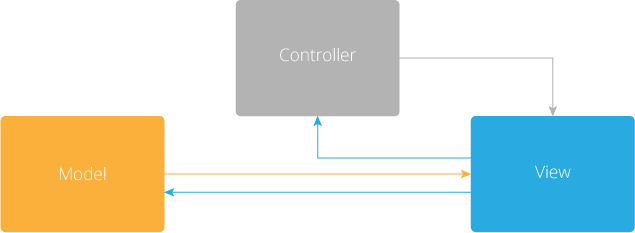
\includegraphics[width=.9\linewidth]{./Abbildungen/model-binding.png}
\end{center}
\item Anwendungszustand und -daten werden von zwei Quellen manipuliert --
unter Umgehung des Controllers
\item Vorteil: Controller wird entlastet
\item Nachteil: Der aktuelle Zustand ist schwer vorhersagbar
\end{itemize}
\subsection*{Unidirektionaler Datenfluss}
\label{sec:org3e38e09}
\begin{center}
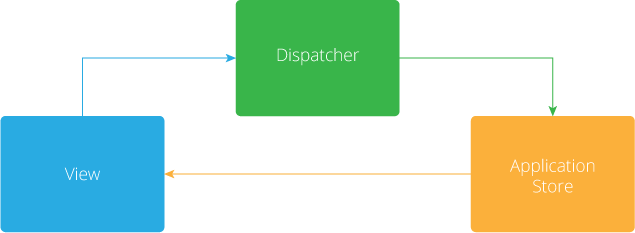
\includegraphics[width=.9\linewidth]{./Abbildungen/unidirectional.png}
\end{center}
\begin{itemize}
\item Änderungen im View löst Aktionen in der Datenkomponente (Application-Store) aus.
\item Diese Änderungen haben Rückwirkungen auf die View-Komponente
\item Kein direkter Zugriff von View auf die Application-Store
\item In React ist der View eine (pure) Funktion der Anwendungsdaten.
\end{itemize}

\section*{Literaturverzeichnis}
\label{sec:org34aa2dc}
\begingroup
\renewcommand{\section}[2]{}%
\printbibliography
\endgroup
\end{document}